\subsection{The Incubator}
%\fbox{Budget: 0.5 page for this subsection}
The different ways of integrating RV monitors into DTs are showcased using the incubator system described in~\cite{Feng&21c}. An overview of this system can be seen at~\cref{subfig:incubator_hw} and~\cref{subfig:incubator_blocks}.
The objective of the incubator is to keep the temperature inside a box close to a target temperature, a task that can be difficult to achieve as more complexities surround the system, such as the possibility of someone opening the lid or the object inside the box releasing heat, are considered.
These considerations have led to the development of a DT for this system~\cite{Feng2022}, which consists of a dynamical model of the physical components of the PT and software components capturing its controller behavior. Additionally, the DT contains a self-adaptation service that reacts to possible changes in the environment and adjusts the incubator's objective as necessary. In order to do this, a MAPE-K architecture is implemented, where a Kalman filter estimates the state of the system and compares it to the empirical data from the sensors. As soon as a deviation is detected, the DT looks at historical data to identify the anomaly and plan accordingly.
The incubator DT has undergone previous verification work, mainly~\cite{Wright2022}, in which the authors propose using reachability analysis to verify that self-adaptations cannot lead to future unsafe states of the incubator.

The approach that we propose in this work differs in the technique used, as we use runtime monitoring to check the truth value of an STL formula that describes the desired behavior of the interaction of the services that belong to the incubator DT.
In order to enable the monitoring of the desired service interaction, a small redesign of the incubator DT architecture was needed.
The self-adaptation service was divided into two different services: anomaly detection, which handles detecting the difference between the expected temperatures and the sensed temperatures, and energy saving, which changes the target temperature to a lower one in case the anomaly detection service has detected an opening of the lid.
Additionally, a runtime monitoring service has also been implemented in the DT, ensuring the correct combined behavior of the anomaly detection and energy saver blocks.
The service monitors the following STL property:
\begin{equation}
	\square(A\implies \lozenge_{[0,3]} S)
\end{equation}
where $A$ stands for the anomaly detection service detecting the opening of the lid and $S$ stands for the energy saver service changing the target temperature. An overview of the interaction of these services and the PT can be seen at~\cref{subfig:incubator_anomaly}.

\begin{figure}[ht]
	\centering
	\begin{subfigure}[t]{0.48\textwidth}
		\centering
		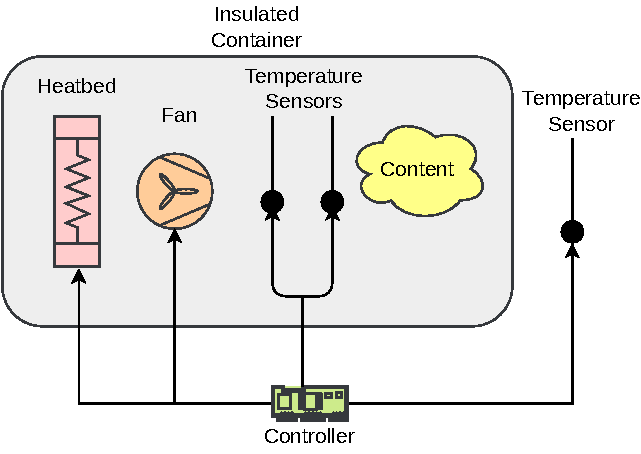
\includegraphics[width=\textwidth]{images/system_hardware.pdf}
		\caption{Hardware overview of the incubator.}
		\label{subfig:incubator_hw}
	\end{subfigure}%
	~
	\begin{subfigure}[t]{0.48\textwidth}
		\centering
		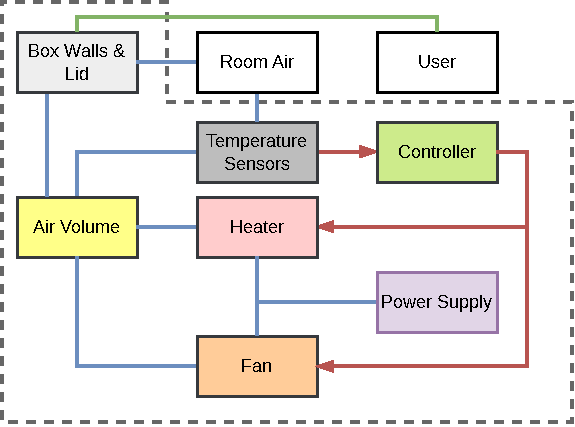
\includegraphics[width=\textwidth]{images/system_block.pdf}
		\caption{Block diagram of the incubator.}
		%The blue connections represent energy interactions, the red connections represent digital information flow, and the green connection represents the user's action by opening and closing the lid. The dashed box represents the system boundary.
		% Outcommented in-depth description of block diagram as it takes up a lot of space.
		\label{subfig:incubator_blocks}
	\end{subfigure}%

	\begin{subfigure}[t]{0.9\textwidth}
		\centering
		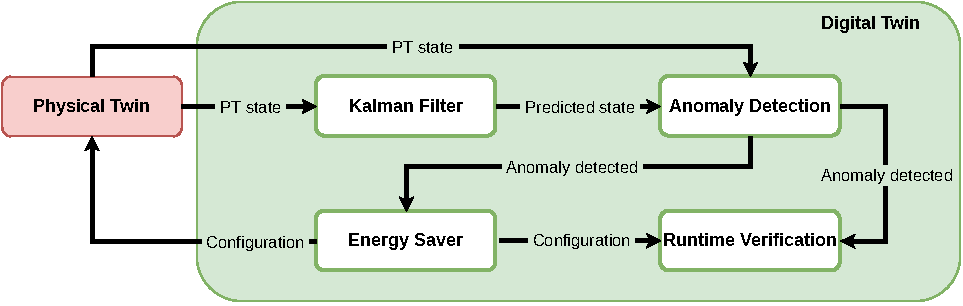
\includegraphics[width=\textwidth]{images/incubator_anomaly_HL.pdf}
		\caption{High-level overview of the DT components relevant to the examples below. Arrows indicate RabbitMQ messages and associated data.}
		\label{subfig:incubator_anomaly}
	\end{subfigure}
	\caption{Overview of the incubator.}
	\label{fig:incubator}
\end{figure}

\begin{comment}
\begin{figure}[htb]
	\centering
	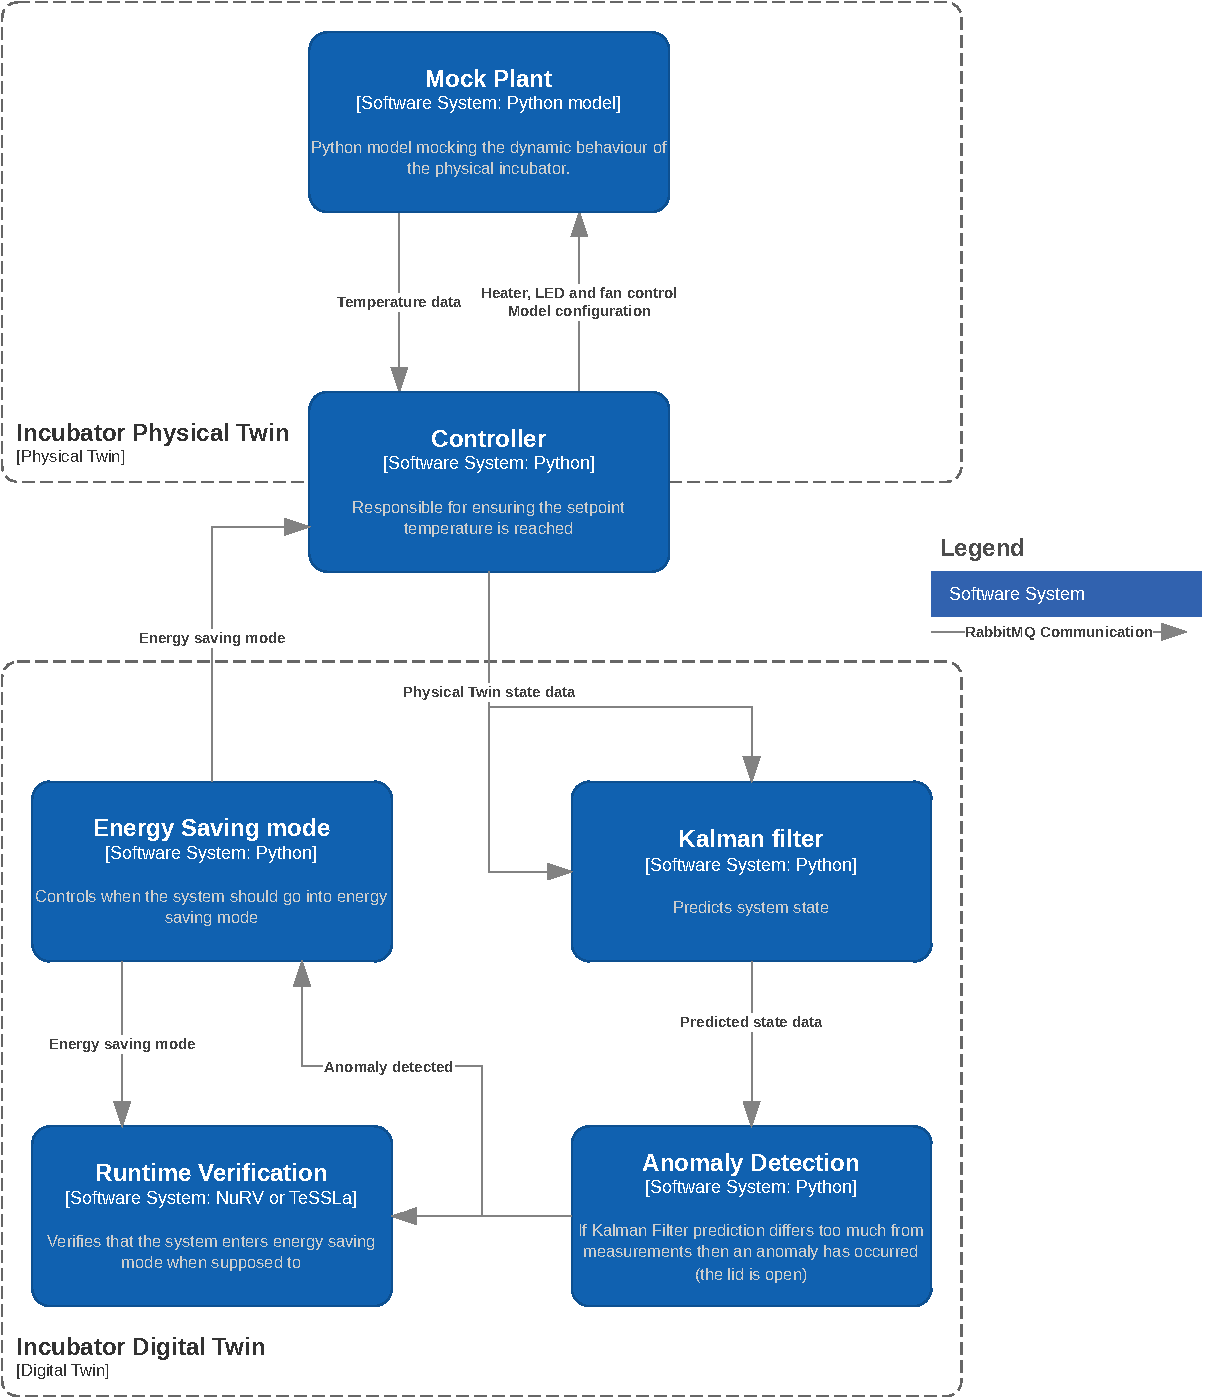
\includegraphics[width=0.9\textwidth]{images/with_energy_saving.pdf}
	\caption{Schematic overview of the incubator DT and PT interaction.}
	\label{fig:incubator}
\end{figure}
\begin{subfigure}[t]{0.48\textwidth}
	\centering
	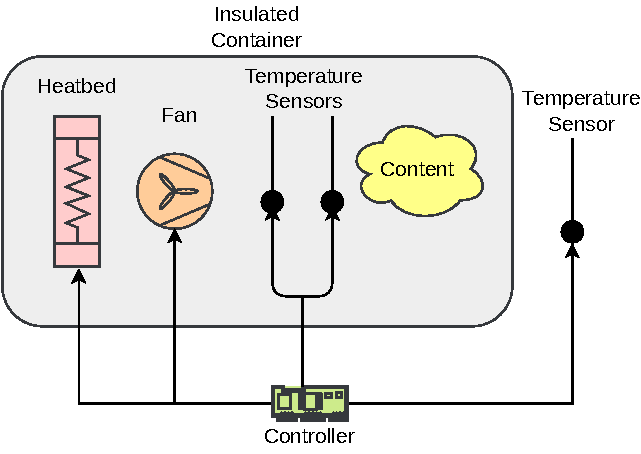
\includegraphics[width=\textwidth]{images/system_hardware.pdf}
	\caption{Hardware components of the incubator.}
	\label{subfig:incubator_hw}
\end{subfigure}%
\end{comment}